\begin{filecontents}{negative.data}
3.7415	6
3.6073	7.7443
4.6561	5.6907
4.4488	6.8871
3.3268	7
4.0829	8.2086
4.9122	4.5121
\end{filecontents}

\begin{filecontents}{allnegative.data}
4.1195	2.28
5.2537	3.4229
4.9122	4.5121
4.1927	4.2979
4.6561	5.6907
3.7415	6
4.4488	6.8871
4.0829	8.2086
3.6073	7.7443
3.3268	7
\end{filecontents}

\begin{filecontents}{positive.data}
1.6927	3
2.8268	2.3393
2.4122	3.385
\end{filecontents}

\begin{filecontents}{allpositive.data}
2.4122	3.385
1	5.1814
2.461	4.78
1.5707	7.8779
1	6.7707
1.8756	5.6136
2.3073	6.6814
1.6927	3
2.8268	2.3393
1.717	3.8243
\end{filecontents}

\begin{filecontents}{w1.data}
5.5    0.0
0.9    9.0
\end{filecontents}

\begin{filecontents}{w2.data}
3.9   0.0
2.5   9.0
\end{filecontents}

\documentclass{beamer}

\mode<presentation>
{
  %\usetheme[secheader]{Madrid}
  \usetheme{Madrid}
  %\usetheme{CCG}
  %\usetheme{Copenhagen} 
  %\useoutertheme{Madrid}
  % or ...

  %\setbeamercovered{transparent}
  % or whatever (possibly just delete it)

}

\usepackage[english]{babel}
% or whatever

\usepackage[latin1]{inputenc}
% or whatever


\usepackage{times}
\usepackage{colortbl}
\usepackage[T1]{fontenc}
% Or whatever. Note that the encoding and the font should match. If T1
% does not look nice, try deleting the line with the fontenc.

\usepackage{graphicx,fancybox}
\usepackage{tabularx}
\usepackage{algorithmic}
\usepackage{tikz}
\usetikzlibrary{shapes,snakes,matrix,arrows,decorations,shadows,plotmarks,calc}


%%%%%%%%%%%%%%%%%%%%%%%%%%%%%%%%%%%%%%%%%%%%%%%%%%%%%%%%%%%%%%%%%%%%%%
%% beamer customization

%modified footer with page number
\makeatletter
\usefoottemplate{%
  \vbox{\tiny%
  \hbox{%
  \setbox\beamer@linebox=\hbox to\paperwidth{%
    \hbox to.5\paperwidth{\hfill\tiny\color{white}\textbf{\insertshortauthor}\hskip.3cm}%
    \hbox to.5\paperwidth{\hskip.3cm\tiny\color{white}\textbf{\insertshorttitle\hfill\insertframenumber}\hskip.3cm}}%
  \ht\beamer@linebox=2.625ex%
  \dp\beamer@linebox=0pt%
  \setbox\beamer@linebox=\vbox{\box\beamer@linebox\vskip1.125ex}%
  \color{black}\hskip-\Gm@lmargin\vrule width.5\paperwidth
  height\ht\beamer@linebox\color{structure}\vrule width.5\paperwidth
  height\ht\beamer@linebox\hskip-\paperwidth% 
  \hbox{\box\beamer@linebox\hfill}\hfill\hskip-\Gm@rmargin}}}
\makeatother

\usenavigationsymbolstemplate{}

\usepackage{babel}

\tikzstyle{ic}=[thick,draw=blue!80,fill=blue!20]
\tikzstyle{hc}=[thick,draw=purple!80,fill=purple!20]
\tikzstyle{fc}=[thick,draw=green!85,fill=green!30]

\tikzstyle{input}=[circle,
                   thick,
                   minimum size=0.6cm,
                   draw=blue!80,
                   fill=blue!20]
\tikzstyle{hidden}=[circle,
                    thick,
                    minimum size=0.6cm,
                    draw=purple!80,
                    fill=purple!20]
\tikzstyle{binary}=[ellipse,
                    thick,
                    minimum size=0.6cm,
                    draw=blue!80,
                    fill=blue!20]
\tikzstyle{feedback}=[circle,
                      thick,
                      minimum size=0.6cm,
                      draw=green!85,
                      fill=green!30]
\tikzstyle{filtered}=[circle,
                      thick,
                      minimum size=0.6cm,
                      draw=gray!70,
                      fill=gray!20]

\tikzstyle{block} = [rectangle, draw=yellow!85, fill=yellow!50,
text width=5em, text centered, rounded corners, minimum height=6em]
\tikzstyle{line} = [draw, -latex']
\tikzstyle{cloud} = [draw=orange!85, ellipse,fill=orange!40,
minimum height=2em,text centered]



\title[] % (optional, use only with long paper titles)
{Driving Semantic Parsing from the World's Response}

%\subtitle{CoNLL 2010}

\author[Clarke, Goldwasser, Chang, Roth] % (optional, use only with lots of authors)
{\textbf{\underline{James Clarke}}, Dan Goldwasser, Ming-Wei Chang, Dan Roth}
% - Use the \inst{?} command only if the authors have different
%   affiliation.

\institute[University of Illinois] % (optional, but mostly needed)
{
  Cognitive Computation Group \\
  University of Illinois at Urbana-Champaign
}
% - Use the \inst command only if there are several affiliations.
% - Keep it simple, no one is interested in your street address.

\date[] % (optional)
{CoNLL 2010}

\subject{Talks}
% This is only inserted into the PDF information catalog. Can be left
% out. 



% If you have a file called "university-logo-filename.xxx", where xxx
% is a graphic format that can be processed by latex or pdflatex,
% resp., then you can add a logo as follows:

% \pgfdeclareimage[height=0.5cm]{university-logo}{university-logo-filename}
% \logo{\pgfuseimage{university-logo}}



% Delete this, if you do not want the table of contents to pop up at
% the beginning of each subsection:
\AtBeginSection[]
{
  \begin{frame}<beamer>
    \frametitle{Outline}
    \tableofcontents[currentsection,currentsubsection]
  \end{frame}
}
\AtBeginSubsection[]
{
  \begin{frame}<beamer>
    \frametitle{Outline}
    \tableofcontents[currentsection,currentsubsection]
  \end{frame}
}

% If you wish to uncover everything in a step-wise fashion, uncomment
% the following command: 

%\beamerdefaultoverlayspecification{<+->}


\begin{document}
% Since this a solution template for a generic talk, very little can
% be said about how it should be structured. However, the talk length
% of between 15min and 45min and the theme suggest that you stick to
% the following rules:  

% - Exactly two or three sections (other than the summary).
% - At *most* three subsections per section.
% - Talk about 30s to 2min per frame. So there should be between about
%   15 and 30 frames, all told.

\section*{Introduction}

\begin{frame}
  \titlepage
\end{frame}

%%%%%%%%%%%%%%%%%%%%%%%%%%%%%%%%%%%%%%%%%%%%%%%%%%%%%%%%%%%%%%%%%%%%%%%%%%%%

\begin{frame}
  \frametitle{What is Semantic Parsing?}
  \begin{tikzpicture}
    % uncomment to draw grid to find where to place nodes
    %\draw[style=help lines, ystep=1, xstep=1] (0,0) grid  (12,8);

  \node at (2.3, 4) [ellipse, draw=blue!80, fill=blue!20, text width=3cm, font=\fontsize{9}{9}\selectfont] (text) {I'd like a coffee with no sugar and just a little milk};

  \node at (2, 1.5) (person) {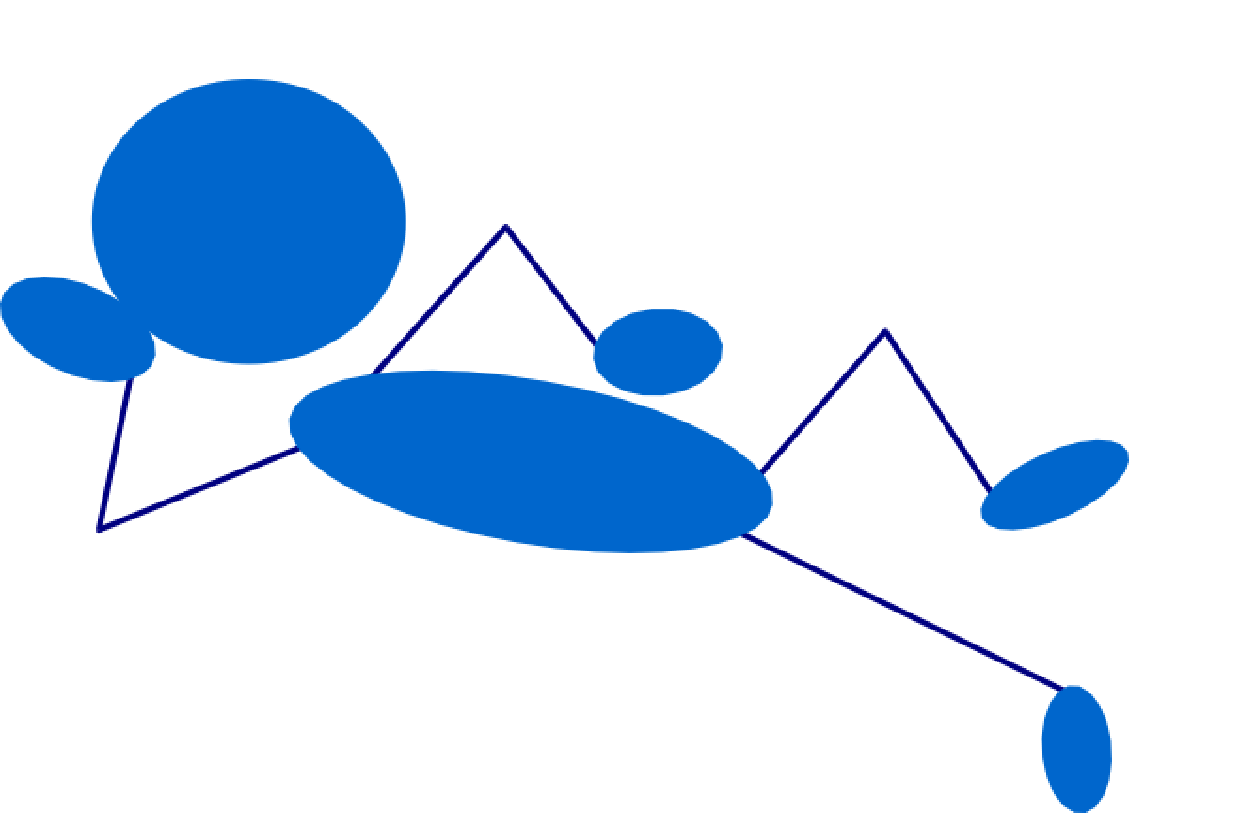
\includegraphics[height=1in]{images/person.pdf}};

  \node at (6, 7) [draw=purple!80, fill=purple!20, font=\ttfamily\fontsize{8.5}{8.5}\selectfont, label=above:{Meaning Representation}] (sp) {make(coffee, sugar=0, milk=0.3)};

  \node<2-> at (10.5, 3) (machine) {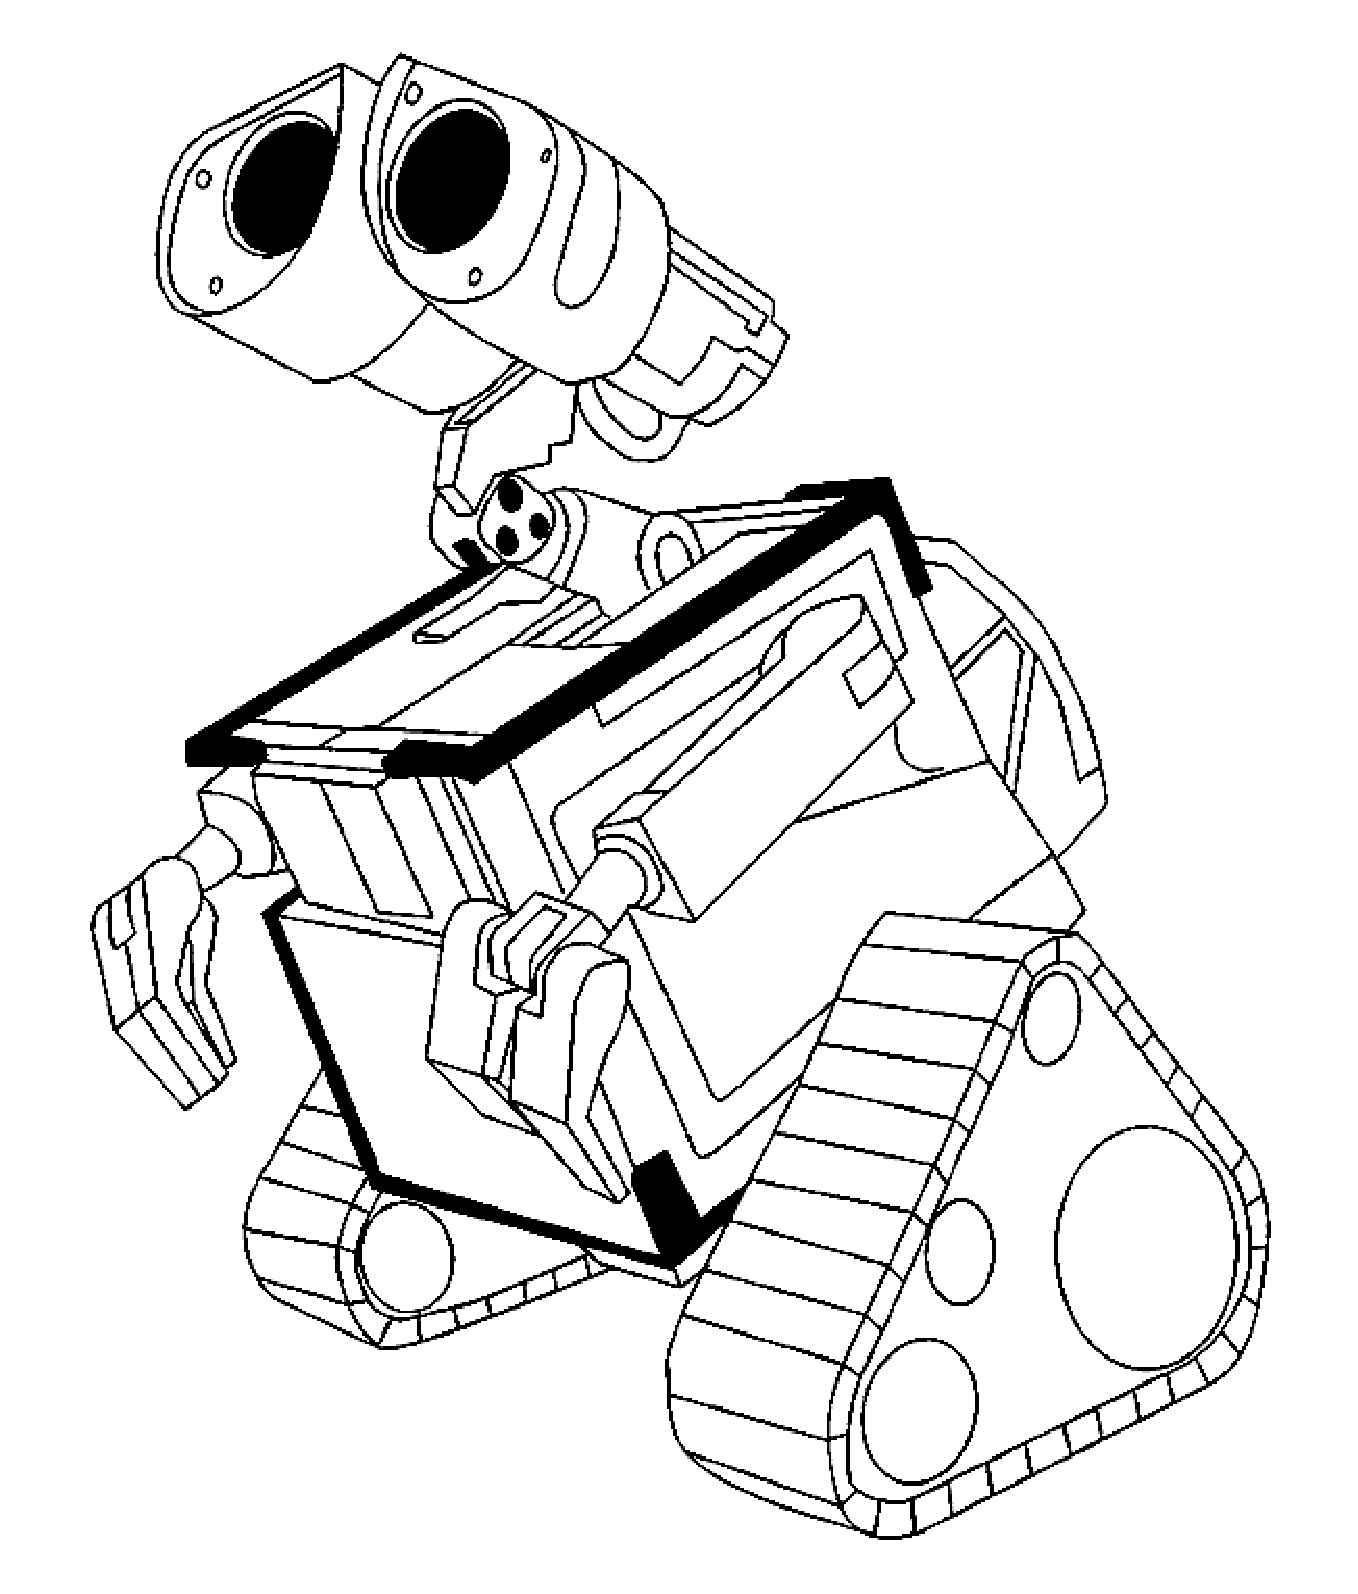
\includegraphics[height=1.7in]{images/wall-e.pdf}};
  
  \node<2-> at (8,3) (coffee) {
\includegraphics[height=0.5in]{images/coffee.pdf}};

  \path[->] (text) edge[very thick, bend left=30] (sp.west);
  \path[->]<2-> (sp.east) edge[very thick, bend left=40] (machine.north);

  
  \end{tikzpicture}
\end{frame}

%%%%%%%%%%%%%%%%%%%%%%%%%%%%%%%%%%%%%%%%%%%%%%%%%%%%%%%%%%%%%%%%%%%%%%%%%%%%

\begin{frame}
  \frametitle{Supervised Learning Problem}
  \begin{center}
    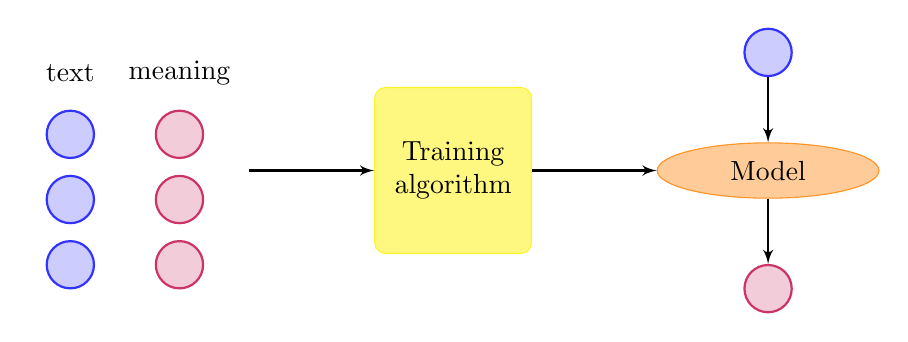
\begin{tikzpicture}
      % rescale nodes if the diagram doesn't fit
      % \tikzset{ every node/.style={scale=0.75} }
      
      \node [block] (init) {Training algorithm};
      
      \matrix[row sep=0.2cm,column sep=0.2cm,ampersand replacement=\&,left of=init,node distance=4cm] (examples) {
        \node {text}; \& \node {meaning}; \\
        \node (x_1)   [input] {};     \&
        \node (y_1)   [hidden] {}; \\
        \node (x_2)   [input] {};     \&
        \node (y_2)   [hidden] {}; \\
        \node (x_2)   [input] {};     \&
        \node (y_2)   [hidden] {}; \\
      };
      

      \node [cloud, right of=init, node distance=4cm, text width=5em] (model) {Model};
      \node (x_t) [input,above of=model,node distance=1.5cm] {};
      \node (y_t) [hidden,below of=model,node distance=1.5cm] {};

      
      \path [line] (examples) edge[thick]  (init);
      \path [line] (init) edge[thick] (model);
      \path [line] (x_t) edge[thick] (model);
      \path [line] (model) edge[thick] (y_t);
    \end{tikzpicture}        
  \end{center}
  Challenges:
  \begin{itemize}
  \item Structured Prediction problem
  \item Model part of the structure as hidden?
  \end{itemize}
\end{frame}

%%%%%%%%%%%%%%%%%%%%%%%%%%%%%%%%%%%%%%%%%%%%%%%%%%%%%%%%%%%%%%%%%%%%%%%%%%%%

\begin{frame}
  \frametitle{Lots of previous work}

  Multiple approaches to the problem:
  \begin{itemize}
  \item \textsc{Krisp} (Kate \& Mooney 2006)
    \begin{itemize}
    \item SVM-based parser using string kernels.
    \end{itemize}
  \item Zettlemoyer \& Collins 2005; Zettlemoyer \& Collins 2007
    \begin{itemize}
    \item Probabilistic parser based on relaxed CCG grammars.
    \end{itemize}
  \item \textsc{Wasp} (Wong \& Mooney 2006; Wong \& Mooney 2007)
    \begin{itemize}
    \item Based on Synchronous CFG.
    \end{itemize}
  \item Ge \& Mooney 2009
    \begin{itemize}
    \item Integrated syntactic and semantic parser.
    \end{itemize}
  \end{itemize}
  \pause
  \textbf{Assumption}: A training set consisting of natural language and meaning
  representation pairs.
\end{frame}

%%%%%%%%%%%%%%%%%%%%%%%%%%%%%%%%%%%%%%%%%%%%%%%%%%%%%%%%%%%%%%%%%%%%%%%%%%%%

\begin{frame}
  \frametitle{Using the World's response}
  \begin{tikzpicture}
    % uncomment to draw grid to find where to place nodes
    %\draw[style=help lines, ystep=1, xstep=1] (0,0) grid  (12,8);

  \node at (2.3, 5) [ellipse, draw=blue!80, fill=blue!20, text width=3cm, font=\fontsize{9}{9}\selectfont] (text) {I'd like a coffee with no sugar and just a little milk};

  \node at (2, 2.7) (person) {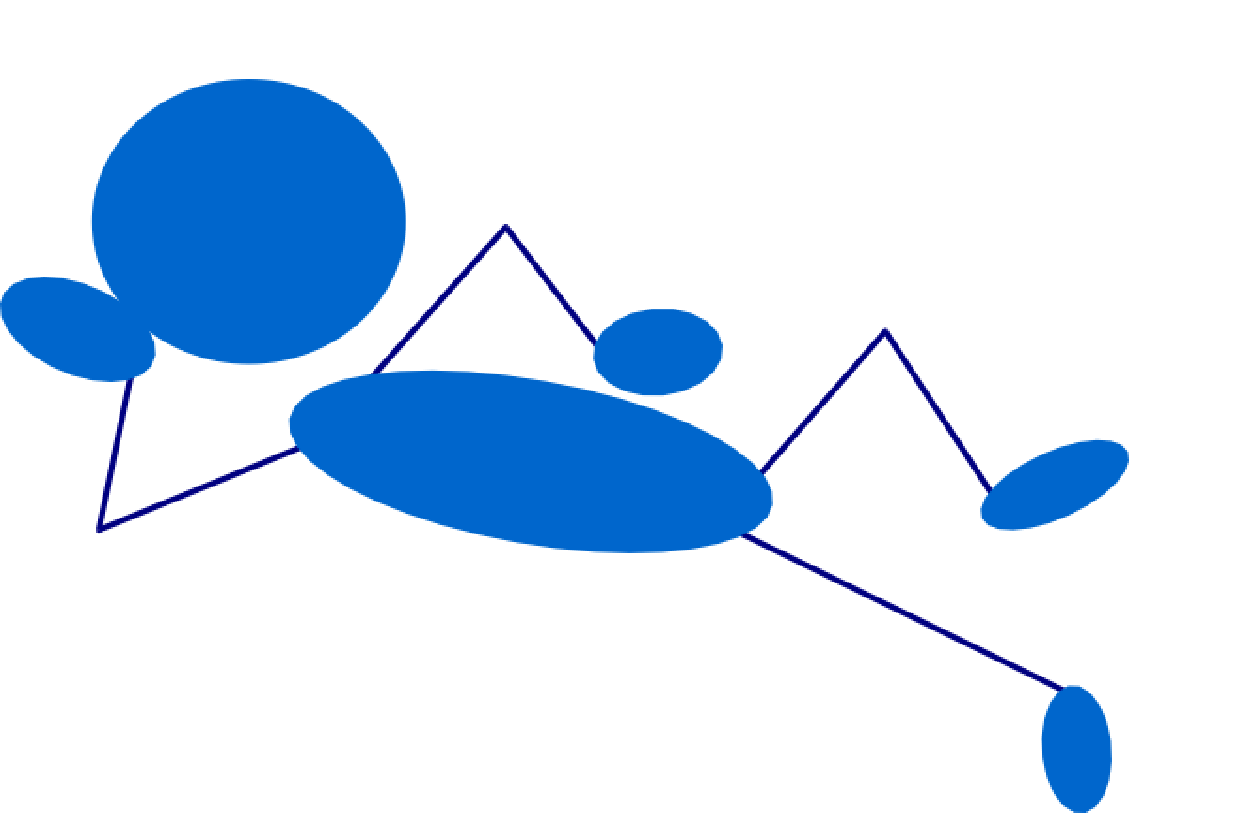
\includegraphics[height=1in]{images/person.pdf}};

  \node at (6, 7) [draw=purple!80, fill=purple!20, font=\ttfamily\fontsize{8.5}{8.5}\selectfont, label=above:{Meaning Representation}] (sp) {make(coffee, sugar=0, milk=0.3)};

  \node at (10.5, 3) (machine) {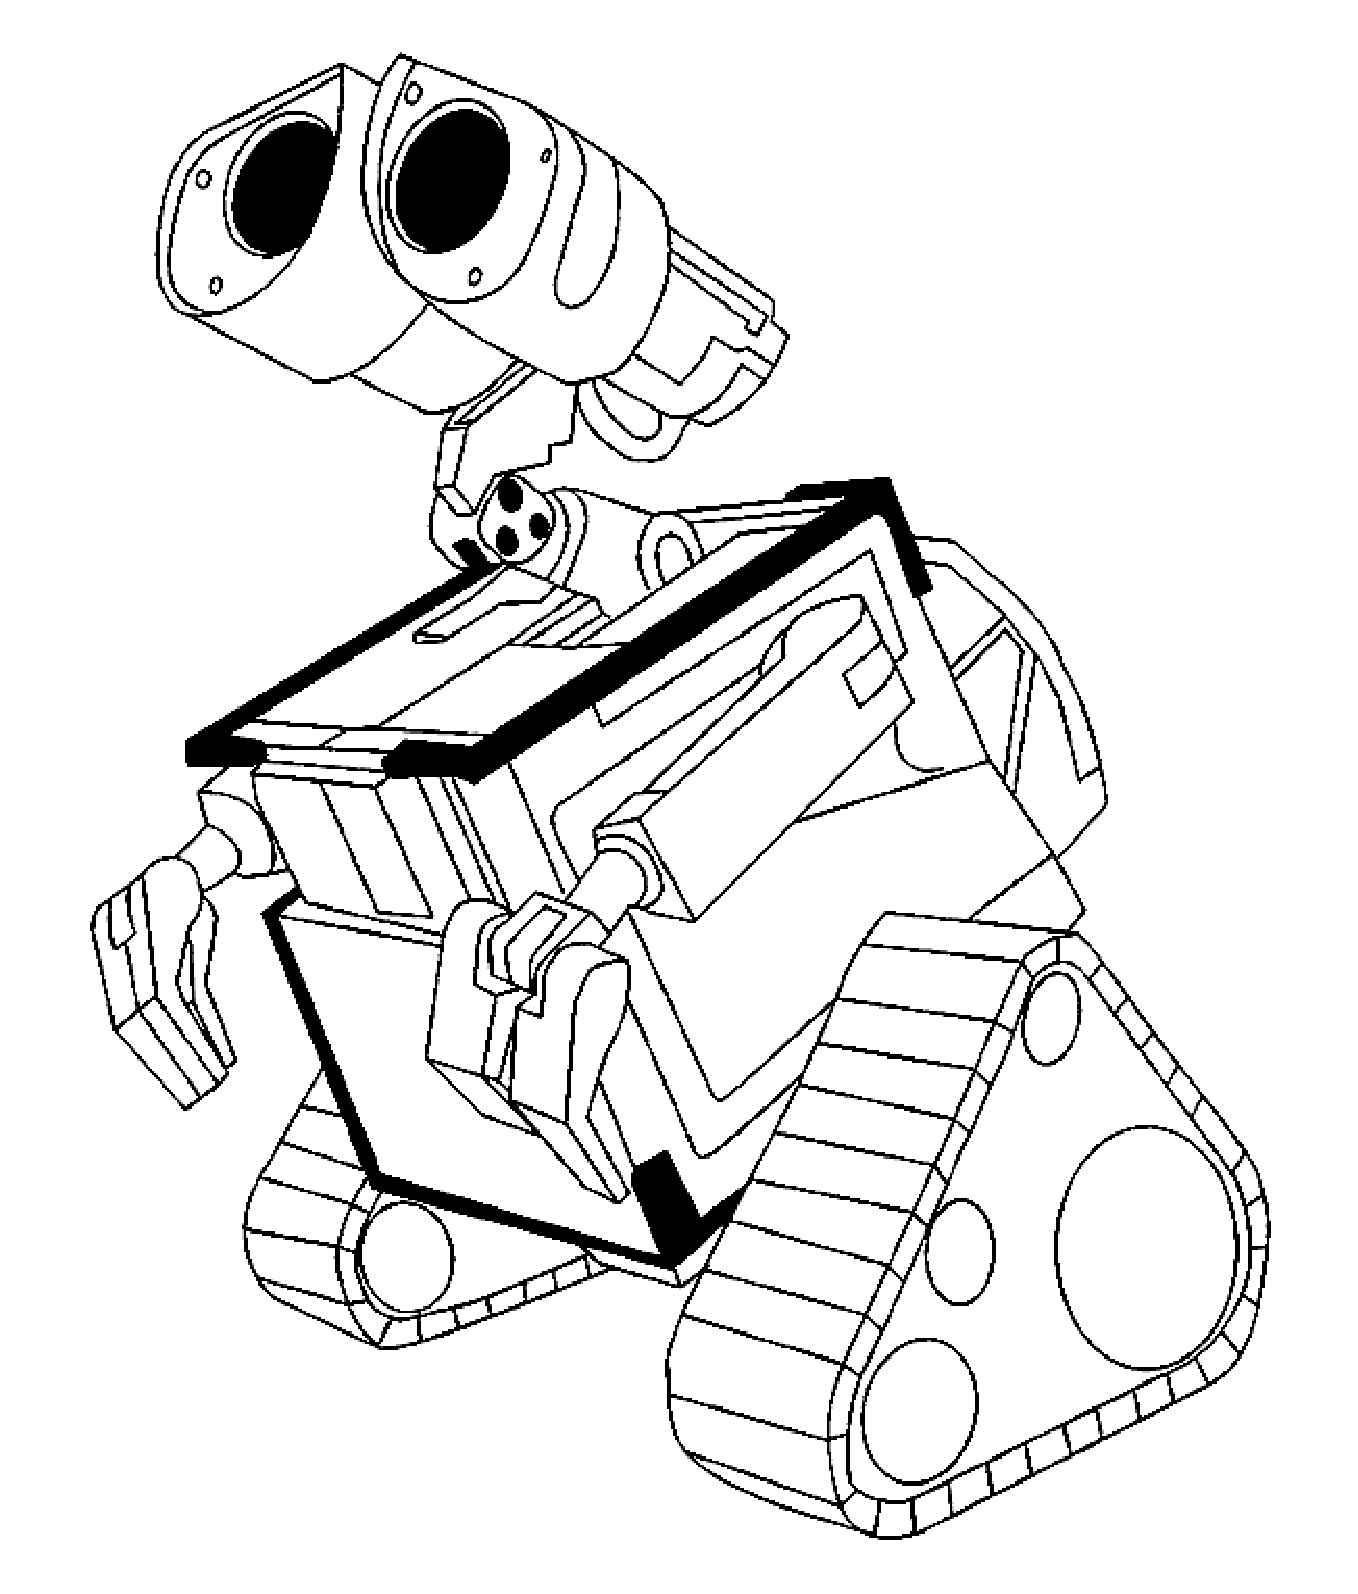
\includegraphics[height=1.7in]{images/wall-e.pdf}};
  
  \node at (8,3) (coffee) {
\includegraphics[height=0.5in]{images/coffee.pdf}};
  \node<2-> at (5,2) [draw=green!85, fill=green!30, circle] (bad) {Bad!}; 
  \node<2-> at (5,4) [draw=green!85, fill=green!30, circle] (good) {Good!}; 

  \path[->] (text) edge[very thick, bend left=30] (sp.west)
  (sp.east) edge[very thick, bend left=40] (machine.north);
  \path[->]<2->
  (coffee.west) edge[very thick] (good)
  (coffee.west) edge[very thick] (bad);
  
  \node<3-> at (5,1.2) [text width=8cm, fill=orange!50] {\textbf{Question:} Can we use feedback based on the response to provide supervision?};
  \end{tikzpicture}
  
\end{frame}
%%%%%%%%%%%%%%%%%%%%%%%%%%%%%%%%%%%%%%%%%%%%%%%%%%%%%%%%%%%%%%%%%%%%%%%%%%%%

\begin{frame}
\frametitle{This work}

\textbf{We aim to}:
\begin{itemize}
\item Reduce the burden of annotation for semantic parsing.
\end{itemize}

\textbf{We focus on}:
\begin{itemize}
\item Using the World's response to learn a semantic parser.
\item Developing new training algorithms to support this learning paradigm.
\item A lightweight semantic parsing model that doesn't require annotated data.
\end{itemize}

\textbf{This results in}:
\begin{itemize}
\item Learning a semantic parser using \alert{zero annotated meaning representations}.
\end{itemize}


\end{frame}

%%%%%%%%%%%%%%%%%%%%%%%%%%%%%%%%%%%%%%%%%%%%%%%%%%%%%%%%%%%%%%%%%%%%%%%%%%%%

\begin{frame}
  \frametitle{Outline}
  \tableofcontents
  % You might wish to add the option [pausesections]
\end{frame}

%%%%%%%%%%%%%%%%%%%%%%%%%%%%%%%%%%%%%%%%%%%%%%%%%%%%%%%%%%%%%%%%%%%%%%%%%%%%

\section{Semantic Parsing}


\begin{frame}
  \frametitle{Semantic Parsing}

  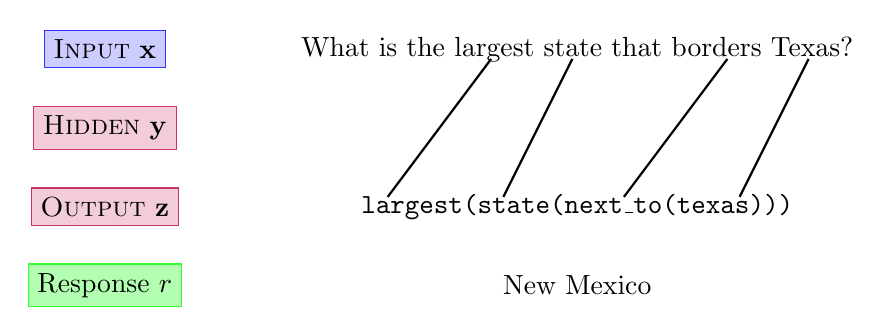
\begin{tikzpicture}
    \node[anchor=west,draw=blue!80, fill=blue!20] (input) {\textsc{Input} $\mathbf{x}$};
    \node[right of=input, node distance=6cm] (sen) {What is the largest state that borders Texas?};
    \node[right of=input, node distance=4cm] (sentence) {};
    \node[right of=sentence, node distance=1cm] (largest) { };
    \node[right of=largest, node distance=1cm] (state) { };
    \node[right of=state,node distance=1cm] (that) { };
    \node[right of=that,node distance=1cm] (borders) { };
    \node[right of=borders,node distance=1cm] (texas) { };
    \node[anchor=west,below of=input, node distance=1cm,draw=purple!80, fill=purple!20] (align) {\textsc{Hidden} $\mathbf{y}$};
    \node[anchor=west,below of=align, node distance=1cm,draw=purple!80, fill=purple!20] (output) {\textsc{Output} $\mathbf{z}$};
    \node[right of=output, node distance=6cm] (lf) {\texttt{largest(state(next\_to(texas)))}};
    \node[right of=output, node distance=3.5cm] (large) { };
    \node[right of=large,node distance=1.5cm] (st) { }; 
    \node[right of=st,node distance=1.5cm] (next) { };
    \node[right of=next,node distance=1.5cm] (tx) { };
    
    \node<4>[anchor=west, below of=output,node distance=1cm,draw=green!80,fill=green!30] (response) {Response $r$};
    \node<4>[right of=response, node distance=6cm] (answer) {New Mexico};
    \path[-,thick] (largest) edge (large)
    (state) edge (st)
    (borders) edge (next)
    (texas) edge (tx);
  \end{tikzpicture}
  \pause
  \begin{center}
    $\mathit{F}:\mathcal{X}\to\mathcal{Z}$
    \begin{displaymath}
      \hat{\mathbf{z}} = \mathit{F_{\mathbf{w}}}(\mathbf{x}) = \operatorname*{arg\,max}_{\mathbf{y}\in\mathcal{Y}, \mathbf{z}\in\mathcal{Z}} \mathbf{w}^T\Phi(\mathbf{x},\mathbf{y}, \mathbf{z})
    \end{displaymath}
  \end{center}
  \pause
  \begin{itemize}
  \item \textbf{Model} The nature of inference and feature functions.
  \item \textbf{Learning Strategy} How we obtain the weights.
  \end{itemize}
\end{frame}

%%%%%%%%%%%%%%%%%%%%%%%%%%%%%%%%%%%%%%%%%%%%%%%%%%%%%%%%%%%%%%%%%%%%%%%%%%%%

\section{Learning}


\begin{frame}[t]
  \frametitle{Learning}
  \textbf{Inputs}:
  \begin{itemize}
  \item Natural language sentences.
  \item $\mathit{Feedback}:\mathcal{X}\times\mathcal{Z}\to\{+1, -1\}$.
  \item \alert{Zero} meaning representations.
  \end{itemize}
  \vspace{2ex}

  \only<2>{
    \begin{exampleblock}{}
     
\begin{displaymath}
  \mathit{Feedback}(\mathbf{x}, \mathbf{z}) = \left\{ \begin{array}{ll}
      +1 & \textrm{if $\mathit{execute}(\mathbf{z}) = r$}\\
      -1 & \textrm{otherwise}
      \end{array}\right.
\end{displaymath}
    \end{exampleblock}
}
\only<3->{
  \textbf{Goal}: A \textbf{weight vector} that scores the correct meaning representation higher
  than all other meaning representations.

  \vspace{2ex}
  \textbf{Response Driven Learning}: \\
  \begin{center}
  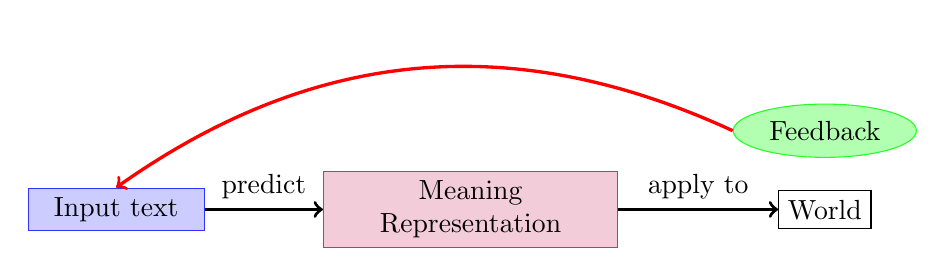
\begin{tikzpicture}
    \node[draw=blue!80, fill=blue!20,,text width=2cm,text centered] (input) {Input text};
    \node[draw=purple!80, fill=purple!20, text width=3.5cm,node distance=4.5cm,right of=input, text centered] (mr) {Meaning\\ Representation};
    \node[draw, node distance=4.5cm, right of=mr, text centered] (world) {World};
    \node[ellipse, above of=world, text centered, fill=green!30, draw=green!85] (feedback) {Feedback};
    \path[->] (input) edge[very thick] node[above] (predict) {predict} (mr)
   (mr) edge[very thick] node[above] (apply) {apply to} (world)
   (feedback.west) edge[very thick,red,bend right=30] (input.north);
    
  \end{tikzpicture}
\end{center}
}
  % \begin{itemize}
  % \item \textsc{Direct} Learn a binary classifier to discriminate between good and bad meaning representations.
  % \item \textsc{Aggressive} Adapt the feedback signal and use structured learning approaches.
  % \end{itemize}
\end{frame}

%%%%%%%%%%%%%%%%%%%%%%%%%%%%%%%%%%%%%%%%%%%%%%%%%%%%%%%%%%%%%%%%%%%%%%%%%%%%

\begin{frame}
  \frametitle{Learning Strategies}
\begin{columns}
\begin{column}{0.45\textwidth}
  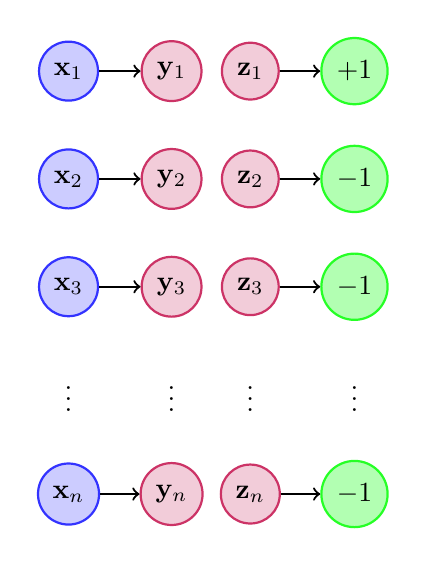
\begin{tikzpicture}
    \matrix[row sep=0.5cm,column sep=0.5cm,ampersand replacement=\&] {
      \node (x_1)   [input] {$\mathbf{x}_1$};     \&
      \node<2-> (y_1)   [hidden] {$\mathbf{y}_1$}; 
      \node<2-> (z_1)   [hidden,right of=y_1] {$\mathbf{z}_1$};    \&
      \node<3-> (r_1)   [feedback] {$+1$};     \\
      \node (x_2)   [input] {$\mathbf{x}_2$};     \&
      \node<2-> (y_2)   [hidden] {$\mathbf{y}_2$}; 
      \node<2-> (z_2)   [hidden,right of=y_2] {$\mathbf{z}_2$};    \&
      \node<3-> (r_2)   [feedback] {$-1$};     \\
      \node (x_3)   [input] {$\mathbf{x}_3$};     \&
      \node<2-> (y_3)   [hidden] {$\mathbf{y}_3$};  
      \node<2-> (z_3)   [hidden,right of=y_3] {$\mathbf{z}_3$};    \& 
      \node<3-> (r_3)   [feedback] {$-1$};     \\
      \node {\vdots}; \& 
      \node<2-> (y_4) [] {\vdots}; 
      \node<2-> (z_4) [right of=y_4] {\vdots}; \&
      \node<3-> {\vdots}; \\
      \node (x_n)   [input] {$\mathbf{x}_n$};     \&
      \node<2-> (y_n)   [hidden] {$\mathbf{y}_n$};  
      \node<2-> (z_n)   [hidden,right of=y_n] {$\mathbf{z}_n$};    \&
      %\node<2-> [dhidden] (yz_n) {$y_n$ \nodepart{lower} $z_n$};\& \&

      \node<3-> (r_n)   [feedback] {$-1$};     \\
    };
    \path[->]<2-> (x_1) edge[thick] (y_1)
(x_2) edge[thick] (y_2)
(x_3) edge[thick] (y_3)
(x_n) edge[thick] (y_n);
\path[->]<3-> (z_1) edge[thick] (r_1)
(z_2) edge[thick] (r_2)
(z_3) edge[thick] (r_3)
(z_n) edge[thick] (r_n);
    
\end{tikzpicture}
\end{column}

\begin{column}{0.5\textwidth}
\begin{block}{}
  \begin{algorithmic}
    \REPEAT
    \FOR{\alert<1>{all input sentences}}
    \STATE
    \alert<2>{Solve the inference problem}
    \STATE 
    \alert<3>{Query $\mathit{Feedback}$ function}
    \ENDFOR
    \STATE \alert<4>{Learn a new $\mathbf{w}$ using feedback}
    \UNTIL {Convergence}
  \end{algorithmic}
\end{block}
\begin{block}{}<2>
  \begin{center}
    $\mathbf{y}, \mathbf{z} = \operatorname*{arg\,max} \mathbf{w}^T \Phi(\mathbf{x},\mathbf{y},\mathbf{z})$
  \end{center}
\end{block}

\end{column}

\end{columns}
 
\end{frame}



%%%%%%%%%%%%%%%%%%%%%%%%%%%%%%%%%%%%%%%%%%%%%%%%%%%%%%%%%%%%%%%%%%%%%%%%%%%%

\subsection{\textsc{Direct} Approach}



\begin{frame}
  \frametitle{\textsc{Direct} Approach}
    \begin{center}
      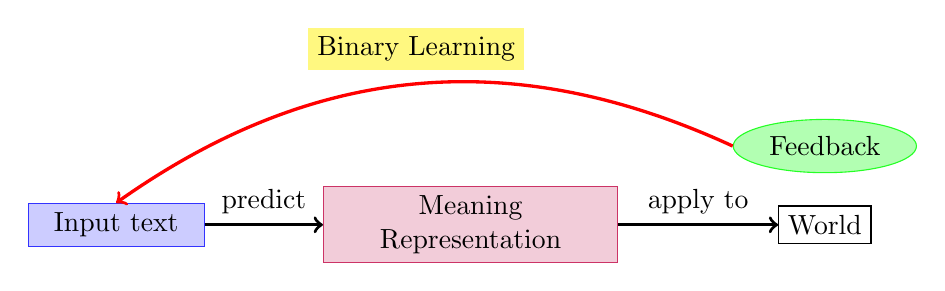
\begin{tikzpicture}
    \node[draw=blue!80, fill=blue!20,,text width=2cm,text centered] (input) {Input text};
    \node[draw=purple!80, fill=purple!20, text width=3.5cm,node distance=4.5cm,right of=input, text centered] (mr) {Meaning\\ Representation};
    \node[draw, node distance=4.5cm, right of=mr, text centered] (world) {World};
    \node[ellipse, above of=world, text centered, fill=green!30, draw=green!85] (feedback) {Feedback};
    \path[->] (input) edge[very thick] node[above] (predict) {predict} (mr)
   (mr) edge[very thick] node[above] (apply) {apply to} (world)
   (feedback.west) edge[very thick,red,bend right=30] node[above=1ex,black,fill=yellow!50] {Binary Learning} (input.north);
        
      \end{tikzpicture}
    \end{center}
    \begin{block}{\textsc{Direct}}
      Learn a binary classifier to discriminate between good and bad meaning representations.      
    \end{block}

\end{frame}
%%%%%%%%%%%%%%%%%%%%%%%%%%%%%%%%%%%%%%%%%%%%%%%%%%%%%%%%%%%%%%%%%%%%%%%%%%%%

\begin{frame}
  \frametitle{\textsc{Direct} Approach}
\begin{columns}
\begin{column}{0.45\textwidth}
  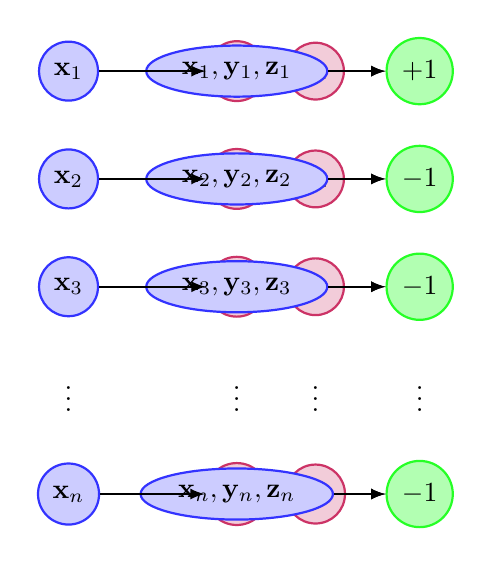
\begin{tikzpicture}[>=latex]
    \matrix[row sep=0.5cm,column sep=0.5cm,ampersand replacement=\&] {
      \node<1> (x_1)   [input] {$\mathbf{x}_1$};     \&
      \node<1> (y_1)   [hidden] {$\mathbf{y}_1$}; 
      \node<1> (z_1)   [hidden,right of=y_1] {$\mathbf{z}_1$};
      \node<2-> (xyz_1) [binary] {$\mathbf{x}_1, \mathbf{y}_1, \mathbf{z}_1$}; \&
      \node (r_1)   [feedback] {$+1$};     \\
      \node<1> (x_2)   [input] {$\mathbf{x}_2$};     \&
      \node<1> (y_2)   [hidden] {$\mathbf{y}_2$}; 
      \node<1> (z_2)   [hidden,right of=y_2] {$\mathbf{z}_2$};
      \node<2-> (xyz_2) [binary] {$\mathbf{x}_2, \mathbf{y}_2, \mathbf{z}_2$}; \&
      \node (r_2)   [feedback] {$-1$};     \\
      \node<1> (x_3)   [input] {$\mathbf{x}_3$};     \&
      \node<1> (y_3)   [hidden] {$\mathbf{y}_3$};  
      \node<1> (z_3)   [hidden,right of=y_3] {$\mathbf{z}_3$};    
      \node<2-> (xyz_3) [binary] {$\mathbf{x}_3, \mathbf{y}_3, \mathbf{z}_3$}; \& 
      \node (r_3)   [feedback] {$-1$};     \\
      \node<1> {\vdots}; \& 
      \node (y_4) [] {\vdots}; 
      \node<1> (z_4) [right of=y_4] {\vdots}; \&
      \node {\vdots}; \\
      \node<1> (x_n)   [input] {$\mathbf{x}_n$};     \&
      \node<1> (y_n)   [hidden] {$\mathbf{y}_n$};  
      \node<1> (z_n)   [hidden,right of=y_n] {$\mathbf{z}_n$};    
      \node<2-> (xyz_n) [binary] {$\mathbf{x}_n, \mathbf{y}_n, \mathbf{z}_n$}; \&
      \node (r_n)   [feedback] {$-1$};     \\
    };
    \path[->]<1> (x_1) edge[thick] (y_1)
(x_2) edge[thick] (y_2)
(x_3) edge[thick] (y_3)
(x_n) edge[thick] (y_n);
\path[->]<1> (z_1) edge[thick] (r_1)
(z_2) edge[thick] (r_2)
(z_3) edge[thick] (r_3)
(z_n) edge[thick] (r_n);
\path[->]<2-> (xyz_1) edge[thick] (r_1)
(xyz_2) edge[thick] (r_2)
(xyz_3) edge[thick] (r_3)
(xyz_n) edge[thick] (r_n);
\end{tikzpicture}
\end{column}
\begin{column}{0.5\textwidth}
\begin{block}{}
\begin{itemize}
\item<1-> Use $(\mathbf{x},\mathbf{y},\mathbf{z})$ as a training example with label from feedback. 
\item<2-> Find $\mathbf{w}$ such that $f\cdot\mathbf{w}^T\Phi(\mathbf{x},\mathbf{y},\mathbf{z}) > 0$
\end{itemize}
\end{block}
% \begin{block}{}<3->
%   \begin{center}
%     $\mathbf{y}, \mathbf{z} = \operatorname*{arg\,max} \mathbf{w}^T \Phi(\mathbf{x},\mathbf{y},\mathbf{z})$
%   \end{center}
% \end{block}

\end{column}
\end{columns}
\end{frame}
%%%%%%%%%%%%%%%%%%%%%%%%%%%%%%%%%%%%%%%%%%%%%%%%%%%%%%%%%%%%%%%%%%%%%%%%%%%%


\begin{frame}
  \frametitle{\textsc{Direct} Approach}
  \begin{columns}
    \begin{column}{0.4\textwidth}
  \begin{tikzpicture}[x=1.7cm,y=0.7cm]
    
  \def\xmin{0}
  \def\xmax{6}
  \def\ymin{0}
  \def\ymax{9}

  %\draw[style=help lines, ystep=1, xstep=1] (\xmin,\ymin) grid  (\xmax,\ymax);
  
  \draw[->, thick] (\xmin,\ymin) -- (\xmax, \ymin);
  \draw[->, thick] (\xmin,\ymin) -- (\xmin,\ymax);

  \draw plot[only marks, mark=*, mark options={fill=blue}, mark size=0.5ex] file {positive.data};
  \draw plot[only marks, mark=*, mark options={fill=red}, mark size=0.5ex] file {negative.data};
  \draw<2->[very thick, purple] plot file {w1.data};

  \coordinate (w1-start) at (5.5, 0.0);
  \coordinate (w1-end) at (0.9, 9.0);
  \coordinate (w1-mid) at ($ (w1-start)!.9!(w1-end) $);
  \coordinate (w1-arrow) at ($ (w1-mid)!0.5cm!90:(w1-end) $);
  \draw<2->[very thick,purple,<-] (w1-arrow) -- (w1-mid) node at (w1-end) [below, black] {$\mathbf{w}$};
  
\end{tikzpicture}
 \end{column}
  \begin{column}{0.5\textwidth}
    \only<1>{\vspace{20ex}\begin{block}{}
    Each point represented by $\Phi(\mathbf{x},\mathbf{y},\mathbf{x})$ normalized by $|\mathbf{x}|$   
    \end{block}}
    \only<2>{\vspace{20ex}\begin{block}{}
        Learn a binary classifier to discriminate between good and bad meaning representations.
    \end{block}}
  \end{column}
  \end{columns}
\end{frame}

%%%%%%%%%%%%%%%%%%%%%%%%%%%%%%%%%%%%%%%%%%%%%%%%%%%%%%%%%%%%%%%%%%%%%%%%%%%%

\begin{frame}
  \frametitle{\textsc{Direct} Approach}
\begin{columns}
\begin{column}{0.45\textwidth}
  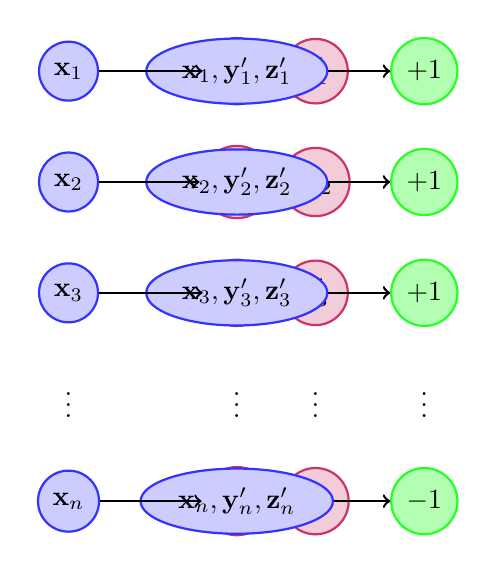
\begin{tikzpicture}
    \matrix[row sep=0.5cm,column sep=0.5cm,ampersand replacement=\&] {
      \node<2-4> (x_1)   [input] {$\mathbf{x}_1$};     \&
      \node<3-4> (y_1)   [hidden] {$\mathbf{y}_1'$}; 
      \node<3-4> (z_1)   [hidden,right of=y_1] {$\mathbf{z}_1'$};    
      \node<5-> (xyz_1) [binary] {$\mathbf{x}_1, \mathbf{y}_1', \mathbf{z}_1'$}; \&
      \node<4-> (r_1)   [feedback] {$+1$};     \\
      \node<2-4> (x_2)   [input] {$\mathbf{x}_2$};     \&
      \node<3-4> (y_2)   [hidden] {$\mathbf{y'}_2$}; 
      \node<3-4> (z_2)   [hidden,right of=y_2] {$\mathbf{z'}_2$};
      \node<5-> (xyz_2) [binary] {$\mathbf{x}_2, \mathbf{y}_2', \mathbf{z}_2'$}; \&
      \node<4-> (r_2)   [feedback] {$+1$};     \\
      \node<2-4> (x_3)   [input] {$\mathbf{x}_3$};     \&
      \node<3-4> (y_3)   [hidden] {$\mathbf{y}_3'$};  
      \node<3-4> (z_3)   [hidden,right of=y_3] {$\mathbf{z}_3'$};
      \node<5-> (xyz_3) [binary] {$\mathbf{x}_3, \mathbf{y}_3', \mathbf{z}_3'$}; \&
      \node<4-> (r_3)   [feedback] {$+1$};     \\
      \node<2-4> {\vdots}; \& 
      \node<3-> (y_4) [] {\vdots}; 
      \node<3-4> (z_4) [right of=y_4] {\vdots}; \&
      \node<4-> {\vdots}; \\
      \node<2-4> (x_n)   [input] {$\mathbf{x}_n$};     \&
      \node<3-4> (y_n)   [hidden] {$\mathbf{y}_n'$};  
      \node<3-4> (z_n)   [hidden,right of=y_n] {$\mathbf{z}_n'$};   
      \node<5-> (xyz_n) [binary] {$\mathbf{x}_n, \mathbf{y}_n', \mathbf{z}_n'$}; \&
      \node<4-> (r_n)   [feedback] {$-1$};     \\
    };
    \path[->]<3-4> (x_1) edge[thick] (y_1)
(x_2) edge[thick] (y_2)
(x_3) edge[thick] (y_3)
(x_n) edge[thick] (y_n);
\path[->]<4> (z_1) edge[thick] (r_1)
(z_2) edge[thick] (r_2)
(z_3) edge[thick] (r_3)
(z_n) edge[thick] (r_n);
\path[->]<5-> (xyz_1) edge[thick] (r_1)    
(xyz_2) edge[thick] (r_2)    
(xyz_3) edge[thick] (r_3)    
(xyz_n) edge[thick] (r_n);
\end{tikzpicture}
\end{column}
\begin{column}{0.5\textwidth}
\begin{block}{}
  \begin{algorithmic}
    \REPEAT
    \FOR{\alert<2>{all input sentences}}
    \STATE
    \alert<3>{Solve the inference problem}
    \STATE 
    \alert<4>{Query $\mathit{Feedback}$ function}
    \ENDFOR
    \STATE \alert<1,5>{Learn a new $\mathbf{w}$ using feedback}
    \UNTIL {Convergence}
  \end{algorithmic}
\end{block}
\begin{block}{}<3>
  \begin{center}
    $\mathbf{y}, \mathbf{z} = \operatorname*{arg\,max} \alert{\mathbf{w}}^T \Phi(\mathbf{x},\mathbf{y},\mathbf{z})$
  \end{center}
\end{block}

\end{column}
\end{columns}
 
\end{frame}


%%%%%%%%%%%%%%%%%%%%%%%%%%%%%%%%%%%%%%%%%%%%%%%%%%%%%%%%%%%%%%%%%%%%%%%%%%%%

\begin{frame}
  \frametitle{\textsc{Direct} Approach}
  \begin{columns}
    \begin{column}{0.4\textwidth}
    \begin{tikzpicture}[x=1.7cm,y=0.7cm]
    
  \def\xmin{0}
  \def\xmax{6}
  \def\ymin{0}
  \def\ymax{9}

  %\draw[style=help lines, ystep=1, xstep=1] (\xmin,\ymin) grid  (\xmax,\ymax);
  
  \draw[->, thick] (\xmin,\ymin) -- (\xmax, \ymin);
  \draw[->, thick] (\xmin,\ymin) -- (\xmin,\ymax);

  \draw<1> plot[only marks, mark=*, mark options={fill=blue}, mark size=0.5ex] file {positive.data};
  \draw<1> plot[only marks, mark=*, mark options={fill=red}, mark size=0.5ex] file {negative.data};
  \draw<2-> plot[only marks, mark=*, mark options={fill=blue}, mark size=0.5ex] file {allpositive.data};
  \draw<2-> plot[only marks, mark=*, mark options={fill=red}, mark size=0.5ex] file {allnegative.data};

  \coordinate (w1-start) at (5.5, 0.0);
  \coordinate (w1-end) at (0.9, 9.0);
  \coordinate (w1-mid) at ($ (w1-start)!.9!(w1-end) $);
  \coordinate (w1-arrow) at ($ (w1-mid)!0.5cm!90:(w1-end) $);
  \draw<1-2>[very thick,purple,<-] (w1-arrow) -- (w1-mid) node at (w1-end) [below, black] {$\mathbf{w}$};
  \draw<1-2>[very thick, purple] plot file {w1.data};

  \coordinate (w2-start) at (3.9, 0.0);
  \coordinate (w2-end) at (2.5, 9.0);
  \coordinate (w2-mid) at ($ (w2-start)!.9!(w2-end) $);
  \coordinate (w2-arrow) at ($ (w2-mid)!0.5cm!90:(w2-end) $);
  \draw<3->[very thick, purple] plot file {w2.data};
  \draw<3->[very thick,purple,<-] (w2-arrow) -- (w2-mid) node at (w2-end) [below left, black] {$\mathbf{w}$};
  \end{tikzpicture}
  \end{column}
  \begin{column}{0.5\textwidth}
    \vspace{-15ex}
    \begin{block}<4->{}
      Repeat until convergence!
    \end{block}
  \end{column}
  \end{columns}

\end{frame}


%%%%%%%%%%%%%%%%%%%%%%%%%%%%%%%%%%%%%%%%%%%%%%%%%%%%%%%%%%%%%%%%%%%%%%%%%%%%

\subsection{\textsc{Aggressive} Approach}


\begin{frame}
  \frametitle{\textsc{Aggressive} Approach}
    \begin{center}
      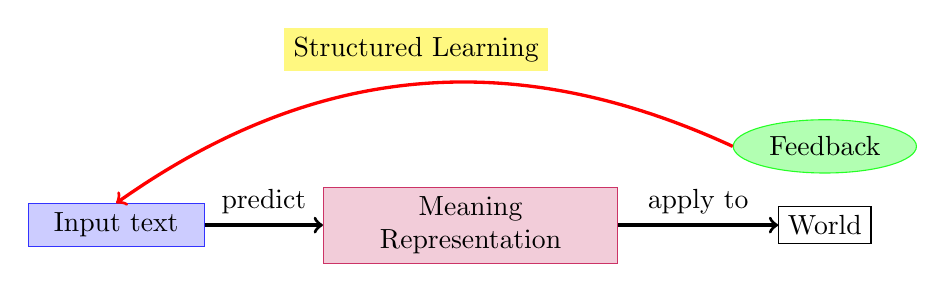
\begin{tikzpicture}
    \node[draw=blue!80, fill=blue!20,,text width=2cm,text centered] (input) {Input text};
    \node[draw=purple!80, fill=purple!20, text width=3.5cm,node distance=4.5cm,right of=input, text centered] (mr) {Meaning\\ Representation};
    \node[draw, node distance=4.5cm, right of=mr, text centered] (world) {World};
    \node[ellipse, above of=world, text centered, fill=green!30, draw=green!85] (feedback) {Feedback};
    \path[->] (input) edge[very thick] node[above] (predict) {predict} (mr)
   (mr) edge[very thick] node[above] (apply) {apply to} (world)
   (feedback.west) edge[very thick,red,bend right=30] node[above=1ex,black,fill=yellow!50] {Structured Learning} (input.north);
 \end{tikzpicture}

    \end{center}
    \begin{block}{\textsc{Aggressive}}
      \begin{itemize}
      \item Positive feedback is a good indicator of the correct meaning representation.
      \item Use data with positive feedback as training data for structured learning.
      \end{itemize}
    \end{block}

\end{frame}

%%%%%%%%%%%%%%%%%%%%%%%%%%%%%%%%%%%%%%%%%%%%%%%%%%%%%%%%%%%%%%%%%%%%%%%%%%%%

\begin{frame}
  \frametitle{\textsc{Aggressive} Approach}
\begin{columns}
\begin{column}{0.45\textwidth}
  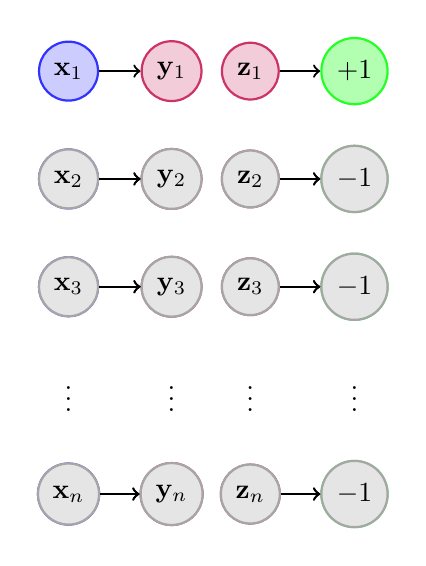
\begin{tikzpicture}
    \matrix[row sep=0.5cm,column sep=0.5cm,ampersand replacement=\&] {
      \node<1-> (x_1)   [input] {$\mathbf{x}_1$};     \&
      \node<1-> (y_1)   [hidden] {$\mathbf{y}_1$}; 
      \node<1-> (z_1)   [hidden,right of=y_1] {$\mathbf{z}_1$};    \&
      \node<1-3> (r_1)   [feedback] {$+1$};     \\
      \node<1-2> (x_2)   [input] {$\mathbf{x}_2$};
      \node<3-> (fx_2)   [filtered] {$\mathbf{x}_2$};     \&
      \node<1-2> (y_2)   [hidden] {$\mathbf{y}_2$}; 
      \node<3-> (fy_2)   [filtered] {$\mathbf{y}_2$}; 
      \node<1-2> (z_2)   [hidden,right of=y_2] {$\mathbf{z}_2$};   
      \node<3-> (fz_2)   [filtered,right of=fy_2] {$\mathbf{z}_2$};    \&
      \node<1-2> (r_2)   [feedback] {$-1$};    
      \node<3> (fr_2)   [filtered] {$-1$};    \\
      \node<1-2> (x_3)   [input] {$\mathbf{x}_3$};
      \node<3-> (fx_3)   [filtered] {$\mathbf{x}_3$};     \&
      \node<1-2> (y_3)   [hidden] {$\mathbf{y}_3$};  
      \node<1-2> (z_3)   [hidden,right of=y_3] {$\mathbf{z}_3$};    
      \node<3-> (fy_3)   [filtered] {$\mathbf{y}_3$};  
      \node<3-> (fz_3)   [filtered,right of=fy_3] {$\mathbf{z}_3$};    \& 
      \node<1-2> (r_3)   [feedback] {$-1$};     
      \node<3> (fr_3)   [filtered] {$-1$};     \\
      \node {\vdots}; \& 
      \node (y_4) [] {\vdots}; 
      \node (z_4) [right of=y_4] {\vdots}; \&
      \node {\vdots}; \\
      \node<1-2> (x_n)   [input] {$\mathbf{x}_n$};     
      \node<3-> (fx_n)   [filtered] {$\mathbf{x}_n$};     \&
      \node<1-2> (y_n)   [hidden] {$\mathbf{y}_n$};  
      \node<1-2> (z_n)   [hidden,right of=y_n] {$\mathbf{z}_n$};    
      \node<3-> (fy_n)   [filtered] {$\mathbf{y}_n$};  
      \node<3-> (fz_n)   [filtered,right of=fy_n] {$\mathbf{z}_n$};   \&
      \node<1-2> (r_n)   [feedback] {$-1$};     
      \node<3> (fr_n)   [filtered] {$-1$};     \\
    };
    \path[->]<1-> (x_1) edge[thick] (y_1);
\path[->]<1-2>(x_2) edge[thick] (y_2)
(x_3) edge[thick] (y_3)
(x_n) edge[thick] (y_n);
\path[->]<3->(fx_2) edge[thick] (fy_2)
(fx_3) edge[thick] (fy_3)
(fx_n) edge[thick] (fy_n);
\path[->]<3>
(fz_2) edge[thick] (fr_2)
(fz_3) edge[thick] (fr_3)
(fz_n) edge[thick] (fr_n);

\path[->]<1-3> (z_1) edge[thick] (r_1);
\path[->]<1-2>
(z_2) edge[thick] (r_2)
(z_3) edge[thick] (r_3)
(z_n) edge[thick] (r_n);
    
\end{tikzpicture}
\end{column}

\begin{column}{0.5\textwidth}
\only<1>{\begin{block}{}
  \begin{algorithmic}
    \REPEAT
    \FOR{all input sentences}
    \STATE
    Solve the inference problem
    \STATE 
    Query $\mathit{Feedback}$ function
    \ENDFOR
    \STATE \alert<1>{Learn a new $\mathbf{w}$ using feedback}
    \UNTIL {Convergence}
  \end{algorithmic}
\end{block}}
\only<2->{
  \begin{block}{}
    \begin{itemize}
    \item<2-> Use items with positive feedback as training data for a structured learner.
    \item<5> Implicitly consider all other meaning representations for these examples as bad.
    \item<5> Find $\mathbf{w}$ such that $\mathbf{w}^T\Phi(\mathbf{x}, \mathbf{y}^*, \mathbf{z}^*) > \mathbf{w}^T\Phi(\mathbf{x},\mathbf{y}',\mathbf{z}')$
    \end{itemize}

  \end{block}
}
\end{column}
\end{columns}
 
\end{frame}

%%%%%%%%%%%%%%%%%%%%%%%%%%%%%%%%%%%%%%%%%%%%%%%%%%%%%%%%%%%%%%%%%%%%%%%%%%%%

\begin{frame}
  \frametitle{\textsc{Aggressive} Approach}
\begin{columns}
\begin{column}{0.45\textwidth}
  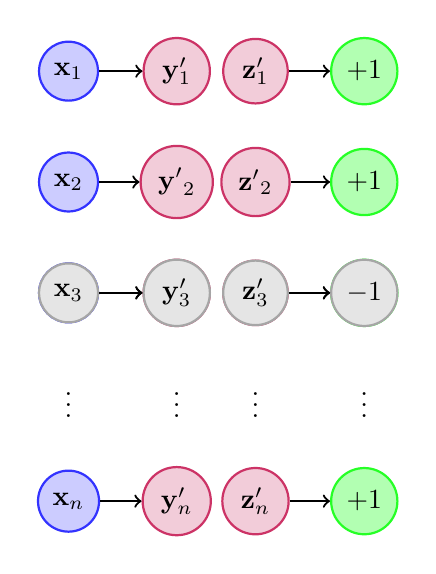
\begin{tikzpicture}
    \matrix[row sep=0.5cm,column sep=0.5cm,ampersand replacement=\&] {
      \node<2-> (x_1)   [input] {$\mathbf{x}_1$};     \&
      \node<3-> (y_1)   [hidden] {$\mathbf{y}_1'$}; 
      \node<3-> (z_1)   [hidden,right of=y_1] {$\mathbf{z}_1'$};  \&
      \node<4-5> (r_1)   [feedback] {$+1$};     \\
      \node<2-> (x_2)   [input] {$\mathbf{x}_2$};     \&
      \node<3-> (y_2)   [hidden] {$\mathbf{y'}_2$}; 
      \node<3-> (z_2)   [hidden,right of=y_2] {$\mathbf{z'}_2$}; \&
      \node<4-5> (r_2)   [feedback] {$+1$};     \\
      \node<2-4> (x_3)   [input] {$\mathbf{x}_3$};
      \node<5-> (fx_3)   [filtered] {$\mathbf{x}_3$};     \&
      \node<3-4> (y_3)   [hidden] {$\mathbf{y}_3'$};  
      \node<3-4> (z_3)   [hidden,right of=y_3] {$\mathbf{z}_3'$};
      \node<5-> (fy_3)   [filtered] {$\mathbf{y}_3'$};  
      \node<5-> (fz_3)   [filtered,right of=fy_3] {$\mathbf{z}_3'$}; \&
      \node<4> (r_3)   [feedback] {$-1$};    
      \node<5> (fr_3)   [filtered] {$-1$};     \\
      \node<2-> {\vdots}; \& 
      \node<3-> (y_4) [] {\vdots}; 
      \node<3-> (z_4) [right of=y_4] {\vdots}; \&
      \node<4-5> {\vdots}; \\
      \node<2-> (x_n)   [input] {$\mathbf{x}_n$};     \&
      \node<3-> (y_n)   [hidden] {$\mathbf{y}_n'$};  
      \node<3-> (z_n)   [hidden,right of=y_n] {$\mathbf{z}_n'$}; \& 
      \node<4-5> (r_n)   [feedback] {$+1$};     \\
    };
    \path[->]<3-> (x_1) edge[thick] (y_1)
(x_2) edge[thick] (y_2)
(x_n) edge[thick] (y_n);
\path[->]<3-4> (x_3) edge[thick] (y_3);
\path[->]<4-5> (z_1) edge[thick] (r_1)
(z_2) edge[thick] (r_2)
(z_n) edge[thick] (r_n);
\path[->]<5->
(fx_3) edge[thick] (fy_3);
\path[->]<4> (z_3) edge[thick] (r_3);
\path[->]<5> (fz_3) edge[thick] (fr_3);

\end{tikzpicture}
\end{column}
\begin{column}{0.5\textwidth}
\begin{block}{}
  \begin{algorithmic}
    \REPEAT
    \FOR{\alert<2>{all input sentences}}
    \STATE
    \alert<3>{Solve the inference problem}
    \STATE 
    \alert<4>{Query $\mathit{Feedback}$ function}
    \ENDFOR
    \STATE \alert<1,5-6>{Learn a new $\mathbf{w}$ using feedback}
    \UNTIL {\alert<7>{Convergence}}
  \end{algorithmic}
\end{block}
\begin{block}{}<3>
  \begin{center}
    $\mathbf{y}, \mathbf{z} = \operatorname*{arg\,max} \alert{\mathbf{w}}^T \Phi(\mathbf{x},\mathbf{y},\mathbf{z})$
  \end{center}
\end{block}
\end{column}
\end{columns}
 
\end{frame}
%%%%%%%%%%%%%%%%%%%%%%%%%%%%%%%%%%%%%%%%%%%%%%%%%%%%%%%%%%%%%%%%%%%%%%%%%%%%

\begin{frame}
  \frametitle{Summary of Learning Strategies}
    \begin{center}
  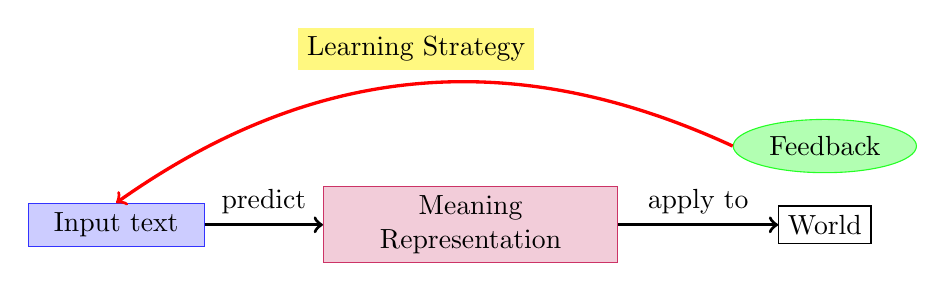
\begin{tikzpicture}
    \node[draw=blue!80, fill=blue!20,,text width=2cm,text centered] (input) {Input text};
    \node[draw=purple!80, fill=purple!20, text width=3.5cm,node distance=4.5cm,right of=input, text centered] (mr) {Meaning\\ Representation};
    \node[draw, node distance=4.5cm, right of=mr, text centered] (world) {World};
    \node[ellipse, above of=world, text centered, fill=green!30, draw=green!85] (feedback) {Feedback};
    \path[->] (input) edge[very thick] node[above] (predict) {predict} (mr)
   (mr) edge[very thick] node[above] (apply) {apply to} (world)
   (feedback.west) edge[very thick,red,bend right=30] node[above=1ex,black,fill=yellow!50] {Learning Strategy} (input.north);

  \end{tikzpicture}
\end{center}
\begin{itemize}
\item \textsc{Direct} Uses both positive and negative feedback as examples to train a binary classifier.
\item \textsc{Aggressive} Adapts the feedback signal and uses only positive feedback to train a structured predictor.
\end{itemize}
\end{frame}
%%%%%%%%%%%%%%%%%%%%%%%%%%%%%%%%%%%%%%%%%%%%%%%%%%%%%%%%%%%%%%%%%%%%%%%%%%%%

\section{Semantic Parsing Model}


\begin{frame}
  \frametitle{Model}
  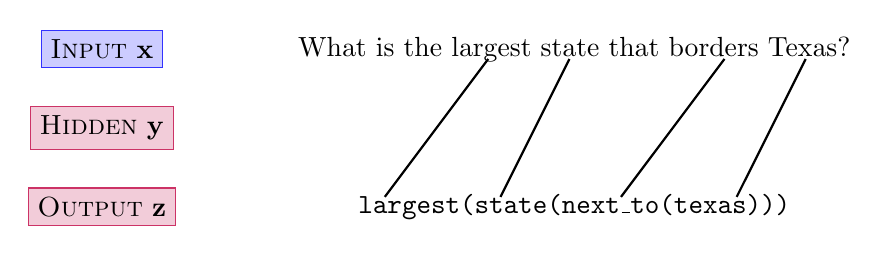
\begin{tikzpicture}
    \node[anchor=west,draw=blue!80, fill=blue!20] (input) {\textsc{Input} $\mathbf{x}$};
    \node[right of=input, node distance=6cm] (sen) {What is the largest state that borders Texas?};
    \node[right of=input, node distance=4cm] (sentence) {};
    \node[right of=sentence, node distance=1cm] (largest) { };
    \node[right of=largest, node distance=1cm] (state) { };
    \node[right of=state,node distance=1cm] (that) { };
    \node[right of=that,node distance=1cm] (borders) { };
    \node[right of=borders,node distance=1cm] (texas) { };
    \node[anchor=west,below of=input, node distance=1cm,draw=purple!80, fill=purple!20] (align) {\textsc{Hidden} $\mathbf{y}$};
    \node[anchor=west,below of=align, node distance=1cm,draw=purple!80, fill=purple!20] (output) {\textsc{Output} $\mathbf{z}$};
    \node[right of=output, node distance=6cm] (lf) {\texttt{largest(state(next\_to(texas)))}};
    \node[right of=output, node distance=3.5cm] (large) { };
    \node[right of=large,node distance=1.5cm] (st) { }; 
    \node[right of=st,node distance=1.5cm] (next) { };
    \node[right of=next,node distance=1.5cm] (tx) { };

    \path[-,thick] (largest) edge (large)
    (state) edge (st)
    (borders) edge (next)
    (texas) edge (tx);
  \end{tikzpicture}
  \vspace{-3ex}
    \begin{center}
    \begin{displaymath}
      \hat{\mathbf{z}} = \mathit{F_{\mathbf{w}}}(\mathbf{x}) = \operatorname*{arg\,max}_{\mathbf{y}\in\mathcal{Y}, \mathbf{z}\in\mathcal{Z}} \mathbf{w}^T\Phi(\mathbf{x},\mathbf{y}, \mathbf{z})
    \end{displaymath}
  \end{center}

  \begin{itemize}
  \item \textbf{First-order}: Map lexical items. largest $\to$ \texttt{largest}
  \item \textbf{Second-order}: Composition. \texttt{next\_to(state($\cdot$))} or \texttt{state(next\_to($\cdot$))}
  \end{itemize}
  Inference procedure leverages the typing information of the domain.
\end{frame}
%%%%%%%%%%%%%%%%%%%%%%%%%%%%%%%%%%%%%%%%%%%%%%%%%%%%%%%%%%%%%%%%%%%%%%%%%%%%
\begin{frame}[plain]
  \frametitle{First-order Decisions}
  \begin{center}
  How many 
  \tikz[baseline,remember picture]{ \node<6-7> [ic,anchor=base] (people) {people};\node<1-5,8->[anchor=base] {people};} 
  live 
  \tikz[baseline,remember picture]{\node<8-9> [ic,anchor=base] (in) {in}; \node<1-7> [anchor=base] {in};}
    the
  \tikz[baseline,remember picture]{\node<3-4> [ic,anchor=base] (st) {state}; \node<1-2,5-> [anchor=base]{state};}
  of
  \tikz[baseline, remember picture]{\node<5> [ic,anchor=base] (texas) {Texas}; \node<1-4,6-> [anchor=base] {Texas};}?
  
  \vspace{5ex}

  \only<2->{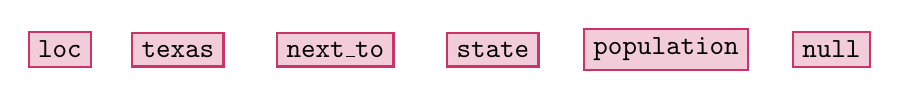
\begin{tikzpicture}[remember picture]
     \node [hc] (loc) {\texttt{loc}}; 
     \node [hc,right of=loc, node distance=1.5cm] (tx) {\texttt{texas}}; 
      \node [hc, right of=tx,node distance=2cm] (il) {\texttt{next\_to}}; 
      \node [hc, right of=il, node distance=2cm] (state) {\texttt{state}};
      \node [hc, right of=state, node distance=2.2cm] (pop) {\texttt{population}}; 
      \node [hc, right of=pop, node distance=2.1cm] (null) {\texttt{null}}; 
    \end{tikzpicture}}
    \begin{tikzpicture}[overlay,remember picture]
      \path<5>[->] (texas) edge[thick] (loc) (texas) edge[thick] (tx) (texas) edge[thick] (il) (texas) edge[thick] (state) (texas) edge[thick] (pop) (texas) edge[thick] (null); 
      \path<3-4>[->] (st) edge[thick] (loc) (st) edge[thick] (tx) (st) edge[thick] (il) (st) edge[thick] (state) (st) edge[thick] (pop) (st) edge[thick] (null); 
      \path<6-7>[->] (people) edge[thick] (loc) (people) edge[thick] (tx) (people) edge[thick] (il) (people) edge[thick] (state) (people) edge[thick] (pop) (people) edge[thick] (null);
      \path<8-9>[->] (in) edge[thick] (loc)  (in) edge[thick] (tx) (in) edge[thick] (il) (in) edge[thick] (state) (in) edge[thick] (pop) (in) edge[thick] (null);
    \end{tikzpicture}
    \begin{columns}
\begin{column}{0.7\textwidth}
  \begin{itemize}
  \item<4-> Use a simple lexicon to bootstrap the process.
  \item<7-> Lexical resources help us move beyond the lexicon.\\
    \texttt{wordnet\_sim(people,population)}
  \item<9-> Context helps disambiguate between choices.
  \end{itemize}
\end{column}

      \begin{column}{0.2\textwidth}
    \begin{footnotesize}
    \begin{block}{}<4->
      $>$ \texttt{texas} \\
      texas\\
      $>$ \texttt{state} \\
      state \\
      $>$ \texttt{population} \\
      population \\
      $>$ \texttt{loc} \\
      in \\
      $>$ \texttt{next\_to} \\
      next \\
      borders \\
      adjacent

    \end{block}

\end{footnotesize}
\end{column}
\end{columns}
\textbf{Goal:} \texttt{population(state(texas))}
\end{center}
  \end{frame}

%%%%%%%%%%%%%%%%%%%%%%%%%%%%%%%%%%%%%%%%%%%%%%%%%%%%%%%%%%%%%%%%%%%%%%%%%%%%
\begin{frame}
  \frametitle{Second-order Decisions}

How do we compose the predicates and constants.

\textbf{Domain dependent:}
\begin{itemize}
\item Encode typing information inherent in the domain into the inference procedure.
\item \texttt{population(state($\cdot$))} vs \texttt{state(population($\cdot$))}
\end{itemize}

\textbf{Features:}
\begin{itemize}
\item Dependency path distance.
\item Word position distance.
\item Predicate ``bigrams''.
\item \texttt{next\_to(state($\cdot$))} vs \texttt{state(next\_to($\cdot$))}
\end{itemize}

\end{frame}

%%%%%%%%%%%%%%%%%%%%%%%%%%%%%%%%%%%%%%%%%%%%%%%%%%%%%%%%%%%%%%%%%%%%%%%%%%%%


\section{Experiments}



%%%%%%%%%%%%%%%%%%%%%%%%%%%%%%%%%%%%%%%%%%%%%%%%%%%%%%%%%%%%%%%%%%%%%%%%%%%%
\begin{frame}
  \frametitle{Evaluation}
  % \begin{block}{Motivation}
  %   Assuming input sentences and feedback function only:
  %   \begin{enumerate}
  %   \item Is it possible to learn a semantic parser \emph{without} meaning
  %     representation annotations?
  %   \item Are there any differences in the two learning algorithms?
  %   \item How much performance do we sacrifice using our model?
  %   \end{enumerate}
  % \end{block}

    \textbf{Domain:}\\
    \textsc{Geoquery}  U.S Geographical Questions.
    \begin{itemize}
    \item Response 250. $(\mathbf{x}, r)$ pairs. Zero meaning representations.
    \item Query 250. $(\mathbf{x})$ sentences.
    \end{itemize}
    \vspace{3ex}
    \textbf{Evaluation metric:}\\
    Accuracy (percentage of meaning representations that
    return the correct answer).

  
\end{frame}



%%%%%%%%%%%%%%%%%%%%%%%%%%%%%%%%%%%%%%%%%%%%%%%%%%%%%%%%%%%%%%%%%%%%%%%%%%%%

\begin{frame}
  \frametitle{Learning Behavior}
  \begin{center}
    \begin{tabular}{|l|c|c|}
      \hline
      Algorithm           & R250    & Q250 \\
      \hline
      \textsc{NoLearn}    & \alert<2>{22.2}     & ---     \\
      \hline\hline
      \textsc{Direct}     & \uncover<6->{\alert<6>{75.2}}     & \uncover<6->{\alert<7>{69.2}}    \\
      \textsc{Aggressive} & \uncover<6->{\alert<6>{82.4}}     & \uncover<6->{\alert<7>{73.2}}    \\
      \hline\hline
      \textsc{Supervised} & 87.6     & \alert<4>{80.4}    \\
      \hline
    \end{tabular}
  \end{center}

  \begin{itemize}
  \only<1-2>{\item<2> \textsc{NoLearn} used to initialize both learning approaches.}
  \only<3-4>{\item<3-4> \textbf{Q:} How good is our model when trained in a fully supervised manner?
  \item<4> \textbf{A:} 80\% on test data. Other supervised methods range from 60\% to 85\% accuracy.}
\only<5-7>{\item<5-7> \textbf{Q:} Is it possible to learn without any meaning representations?
  \item<6-7> \textbf{A:} Yes!
  \item<6-7> \textbf{A:} Learns to cover more of the Response data set.
  \item<6-7> \textbf{A:} And only 7\% below the \textsc{Supervised} upper bound.}
  \end{itemize}
\end{frame}

%%%%%%%%%%%%%%%%%%%%%%%%%%%%%%%%%%%%%%%%%%%%%%%%%%%%%%%%%%%%%%%%%%%%%%%%%%%%

\begin{frame}
  \frametitle{Learning Behavior}
  
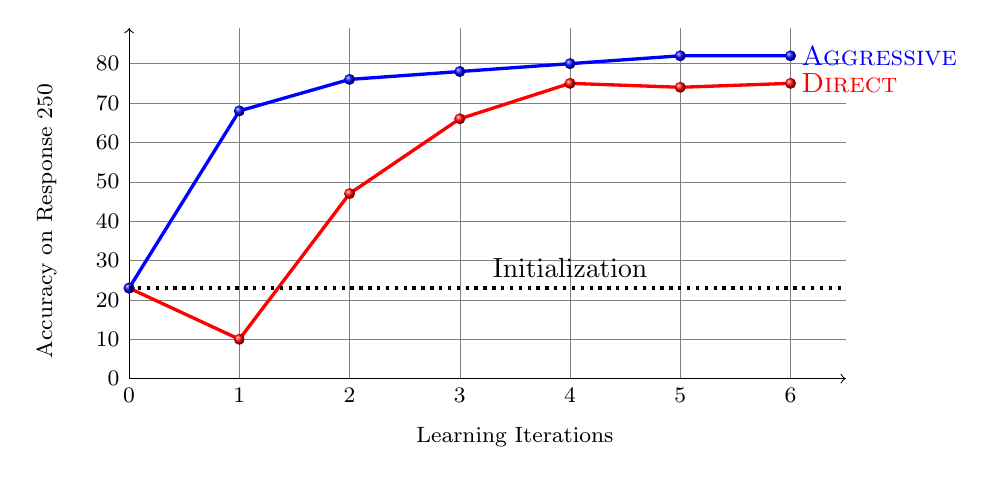
\begin{tikzpicture}[x=1.4cm, y=0.05cm]
  \def\xmin{0}
  \def\xmax{6.5}
  \def\ymin{0}
  \def\ymax{89}

  % grid
  \draw[style=help lines, ystep=10, xstep=1] (\xmin,\ymin) grid
  (\xmax,\ymax);

  \draw[->] (\xmin,\ymin) -- (\xmax, \ymin);
  \draw[->] (\xmin,\ymin) -- (\xmin,\ymax);

  %labels      
	\node[below=0.5cm] at (3.5, \ymin) {\footnotesize{Learning Iterations}};
	\node[rotate=90, above=0.8cm] at (\xmin, 40) {\footnotesize{Accuracy on Response 250}};

  % xticks and yticks
  \foreach \x in {0,1,...,6}
    \node at (\x, \ymin) [below] {\footnotesize{\x}};
  \foreach \y in {0,10,...,80}
    \node at (\xmin,\y) [left] {\footnotesize{\y}};

  \draw[very thick, red] plot[mark=ball, ball color=red] coordinates {(0, 23) (1,10) (2,47) (3, 66) (4, 75) (5, 74) (6, 75)} node [right] {\textsc{Direct}};

  \draw[very thick, blue] plot[mark=ball] coordinates {(0,23) (1,68) (2,76) (3,78) (4,80) (5,82) (6,82)} node [right] {\textsc{Aggressive}};;
  \draw[very thick, style=dotted] plot coordinates {(\xmin, 23) (\xmax, 23)} node at (4, 23) [above] {Initialization};
\end{tikzpicture}
\vspace{-2ex}
\begin{itemize}
\item \textsc{Aggressive} correctly interprets 16\% that \textsc{Direct} does not. 9\% vice-versa. Leaving only 9\% incorrect.
\end{itemize}
\end{frame}

%%%%%%%%%%%%%%%%%%%%%%%%%%%%%%%%%%%%%%%%%%%%%%%%%%%%%%%%%%%%%%%%%%%%%%%%%%%%
% \begin{frame}
%   \frametitle{Results}
%   \begin{center}
%     \begin{tabular}{|l|c|c|}
%       \hline
%       Algorithm           & \# LF    & Q250 \\
%       \hline
%       \textsc{Aggressive} & 0     & 73.2    \\
%       \hline\hline
%       \textsc{Supervised} & 250     & 80.4    \\
%       \hline\hline
%       \textsc{W\&M 2006}  & $\sim$ 310   & $\sim$ 60.0   \\
%       \textsc{W\&M 2007}  & $\sim$ 310   & $\sim$ 75.0   \\
%       \hline\hline
%       \textsc{Z\&C 2005}  & 600    & 79.29 \\
%       \textsc{Z\&C 2007}  & 600    & 86.07 \\
%       \textsc{W\&M 2007}  & 800    & 86.59 \\
%       \hline
%     \end{tabular}    
%   \end{center}
%   \begin{itemize}
%   \item \textsc{Aggressive} outperforms some supervised techniques.
%   \item Our model trained in a supervised manner still competitive with other approaches.
%   \end{itemize}
% \end{frame}

%%%%%%%%%%%%%%%%%%%%%%%%%%%%%%%%%%%%%%%%%%%%%%%%%%%%%%%%%%%%%%%%%%%%%%%%%%%%

\begin{frame}
  \frametitle{Learning from Indirect Supervision}
  Similar to indirect learning protocols:
  \begin{itemize}
  \item Learning a binary classifier with ``hidden explanation''. Supervision
    only required for binary data. No labeled structures. NAACL 2010 (Chang,
    Goldwasser, Roth, Srikumar 2010a).
  \item Structured learning with binary and structured labels. Mix of
    supervision for binary data and structured data. Binary label indicates
    whether input has a ``good'' structure. ICML 2010 (Chang, Goldwasser, Roth,
    Srikumar 2010b).
  \end{itemize}
\end{frame}

%%%%%%%%%%%%%%%%%%%%%%%%%%%%%%%%%%%%%%%%%%%%%%%%%%%%%%%%%%%%%%%%%%%%%%%%%%%%
\begin{frame}
  \frametitle{Conclusions}
  \textbf{Contributions:}
  \begin{itemize}
  \item Response Driven Learning. A new learning paradigm that doesn't rely on
    annotated meaning representations. Supervised at the response level. Natural
    supervision signal.
  \item Two learning algorithms capable of working within response driven
    learning.
  \item A shallow semantic parsing model.
  \end{itemize}

  \vspace{1ex}
  \textbf{Future work:}
  \begin{itemize}
  \item Can we combine the two learning algorithms?
  \item Other semantic parsing domains?
  \item Response driven learning for other tasks?
  \end{itemize}
\end{frame}
%%%%%%%%%%%%%%%%%%%%%%%%%%%%%%%%%%%%%%%%%%%%%%%%%%%%%%%%%%%%%%%%%%%%%%%%%%%%
%%%%%%%%%%%%%%%%%%%%%%%%%%%%%%%%%%%%%%%%%%%%%%%%%%%%%%%%%%%%%%%%%%%%%%%%%%%%
%%%%%%%%%%%%%%%%%%%%%%%%%%%%%%%%%%%%%%%%%%%%%%%%%%%%%%%%%%%%%%%%%%%%%%%%%%%%
%%%%%%%%%%%%%%%%%%%%%%%%%%%%%%%%%%%%%%%%%%%%%%%%%%%%%%%%%%%%%%%%%%%%%%%%%%%%
%%%%%%%%%%%%%%%%%%%%%%%%%%%%%%%%%%%%%%%%%%%%%%%%%%%%%%%%%%%%%%%%%%%%%%%%%%%%
%%%%%%%%%%%%%%%%%%%%%%%%%%%%%%%%%%%%%%%%%%%%%%%%%%%%%%%%%%%%%%%%%%%%%%%%%%%%
%%%%%%%%%%%%%%%%%%%%%%%%%%%%%%%%%%%%%%%%%%%%%%%%%%%%%%%%%%%%%%%%%%%%%%%%%%%%

\end{document}